% Column-width variant of ../../tese/Introduction/figures/system_overview.tex for the extended abstract
% (standalone; compile with pdflatex and include system_overview_column.pdf)
\documentclass[tikz, border=2pt]{standalone}
\usepackage[T1]{fontenc}
\usepackage{helvet}
\renewcommand{\familydefault}{\sfdefault}
\usetikzlibrary{arrows.meta, positioning, calc}

\definecolor{rosline}{RGB}{34, 49, 79}
\definecolor{vehfill}{RGB}{253, 242, 228}
\definecolor{vehline}{RGB}{214, 140, 60}

\begin{document}
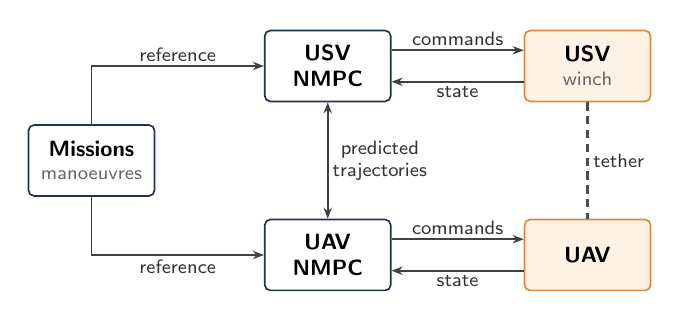
\begin{tikzpicture}[
    box/.style={draw=#1, fill=white, rounded corners=2pt, align=center, minimum width=1.6cm, minimum height=0.9cm,
                inner sep=2pt, font=\footnotesize, line width=0.6pt},
    box/.default=rosline,
    flow/.style={-{Stealth[length=4pt]}, line width=0.6pt, black!75},
    both/.style={{Stealth[length=4pt]}-{Stealth[length=4pt]}, line width=0.6pt, black!75},
    lbl/.style={font=\scriptsize, black!80, inner sep=1.5pt, align=center},
]
\node[box] (exec) at (0, 0) {\textbf{Missions}\\[-1pt]\textcolor{black!60}{\scriptsize manoeuvres}};
\node[box] (usvc) at (3.0, 1.2) {\textbf{USV}\\\textbf{NMPC}};
\node[box] (uavc) at (3.0, -1.2) {\textbf{UAV}\\\textbf{NMPC}};
\node[box=vehline, fill=vehfill] (usv) at (6.3, 1.2) {\textbf{USV}\\[-1pt]\textcolor{black!60}{\scriptsize winch}};
\node[box=vehline, fill=vehfill] (uav) at (6.3, -1.2) {\textbf{UAV}};

\draw[flow] (exec.north) |- node[lbl, above, pos=0.75] {reference} (usvc.west);
\draw[flow] (exec.south) |- node[lbl, below, pos=0.75] {reference} (uavc.west);
\draw[both] (usvc) -- node[lbl, right] {predicted\\trajectories} (uavc);
\draw[flow] (usvc.east |- 0, 1.4) -- node[lbl, above] {commands} (usv.west |- 0, 1.4);
\draw[flow] (usv.west |- 0, 1.0) -- node[lbl, below] {state} (usvc.east |- 0, 1.0);
\draw[flow] (uavc.east |- 0, -1.0) -- node[lbl, above] {commands} (uav.west |- 0, -1.0);
\draw[flow] (uav.west |- 0, -1.4) -- node[lbl, below] {state} (uavc.east |- 0, -1.4);
\draw[line width=1.2pt, black!70, densely dashed] (usv) -- node[lbl, right] {tether} (uav);
\end{tikzpicture}
\end{document}
